\newpage
%\null
%\cleardoublepage



%************************************************************************************************
% Kap.3 Mathematische Modellbildung
%************************************************************************************************
\unit[1]{ms}
\chapter{Mathematische Modellbildung}
\label{chap:modellbildung}

\section{Das System}
\label{chap:system}
Der vorliegenden Simulationsstudie wird folgendes, in Abb. \ref{fig:aufbau_system} dargestellen Systems zugrunde gelegt.
\begin{figure}[!h]
	\centering
	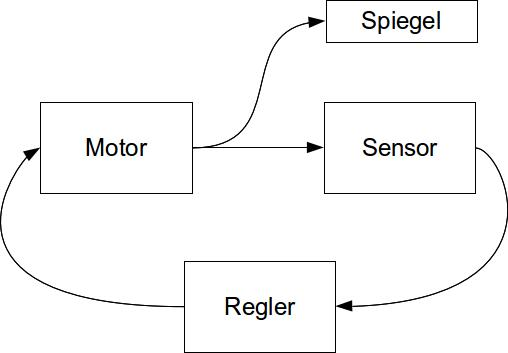
\includegraphics[width=0.6\textwidth]{System_Aufbau.jpg}
	\caption{Allgemeiner Aufbau des simulierten Systems}
	\label{fig:aufbau_system}
\end{figure}

\section{Der Spiegel}
\label{chap:spiegel}
Der Spiegel ist das Bauteil, welches durch den Gleichstrommotor bewegt werden soll.
F�r die Integration in die Simulation m�ssen vorab einige Berechnungen angestellt werden.
Als erstes wird die ben�tigte Beschleunigung berechnet, die mit einem Drehmoment auf den Spiegel �bertragen werden muss, um den Spiegel mit seinem Tr�gheitsmoment �ber 
seinen maximalen Ablenkwinkel zu bewegen.

Dabei werden folgende Vorgaben zu Grunde gelegt:
\begin{itemize}
\item Maximale Ablenkung von $\phi$ = \unit[20}{�} \approx \unit[0,349]{rad}
\item Maximale Zeit f�r Ablenkung \unit[1]{ms}
\item Lineares Modell
\end{itemize}
Berechnung der Winkelgeschwindigkeit:
\begin{center}
\begin{equation}
\label{equ:lineares_motor_model}
\Delta \phi = \unit[20]{�} = \unit[0,349]{rad}\\
\Delta t = \unit[1]{ms} = \unit[0,001]{s}\\
\omega = \frac {\Delta \phi}{\Delta t} = \frac {\unit[0,349]{rad}}{\unit[0,001]{s}} = \unit[349]{rad/s}\\
\end{equation}
\end{center}

Es ergibt sich eine Druchschnittswinkelgeschwindigkeit von \unit[349]{rad/s}, um einen Winkel von \unit[20}{�} in \unit[1]{ms} zu �berfahren.
Dies w�rde aber eine Anfangs- und Endgeschwindigkeit voraussetzen. Da der Spiegel aber aus einer Ruhelage beschleunigt und wieder in einer Ruhelage enden soll, 
wird ein linearer Verlauf der Geschwindigkeit von $\omega = \unit{0}{rad/s}$ und der doppelten Durchschnittsgeschwindigkeit $\omega = \unit{698}{rad/s}$ bei der H�lfte der 
Strecke und bei der Endposition wieder $\omega = \unit{0}{rad/s}$ der zu fahrenden Strecke angenommen. 
Daraus folgt eine Beschleunigung von:
\begin{center}
\begin{equation}
\label{equ:max_alpha_motor}
\Delta \omega = \unit[698]{rad/s}\\
\Delta t = \unit[0,5]{ms} = \unit[0,0005]{s}\\
\\
\alpha = \frac {\Delta \omega}{\Delta t} = \frac {\unit{698}{rad/s}}{\unit{0,0005}{s}} = \unit{1,396 *10^6}{rad/s^2}\\
\end{equation}
\end{center}
Der Spiegel erf�hrt zu Beginn der Regelung eine Beschleunigung von $\alpha = \unit{1,396 *10^6}{rad/s^2}$ um nach der H�lfte der Zeit, also nach \unit[0,5]{ms} wieder mit 
dem gleichen Betrag der Beschleunigung abgebremst zu werden.

Modell f�r den Spiegel:
\begin{itemize}
\item Durchmesser: \unit[12]{mm} --> Radius: R = \unit[6]{mm}
\item H�he: h = \unit[2]{mm}
\item Gewicht: m = \unit[10]{g}
\end{itemize}

Das Tr�gheitsmoment des Spiegels betr�gt demnach: 
\begin{center}
\begin{equation}
\label{equ:J_spiegel}
J = \frac {1} {4} * m * R^2 + \frac{1}{12} * m * h^2\\
J = \frac {1} {4} * \unit[10e-3]{kg} * (\unit[[6e-3]{m})^2 + \frac{1}{12} * \unit[10e-3]{kg} * (\unit[[2e-3]{m})^2\\
J = \unit[93,3e-9]{kgm^2}
\end{equation}
\end{center}

Aus den oben berechneten Daten ergibt sich ein Lastmoment von:
\begin{center}
\begin{equation}
\label{equ:M_last}
M_L = J * \alpha\\
M_L = \unit[93,3e-9]{kgm^2} * \unit[1,396e6]{rad/s^2} \\
M_L = \unit[130,25e-3]{Nm}
\end{equation}
\end{center}

Theoretische Maximale Leistung eines Gleichstrommotors:
\begin{center}
\begin{equation}
\label{equ:max_leistung_motor}
P = M_L * \omega\\
P = \unit[130,25 * 10^{-3}]{Nm} * \unit[698]{rad/s} \\
P = \unit[91]{W}
\end{equation}
\end{center}

\section{Der Motor}
\label{chap:motor}
In der Regel werden Laserablenkespiegel �ber einen Galvo gesteuert. Bei der Bearbeitung dieser Simulationsstudie ergaben sich Probleme, Informationen �ber die Ansteuerung
solcher Galvos zu bekommen. Insofern wird die Simulationsstudie auf der Ansteuerung eines Gleichstrommotors beruhen. Aber auch hierbei konnten jedoch keine Informationen 
�ber die Gleichstrommotorparameter $K_M\phi$ und der Reibungskonstanten bei verschiedenen Herstellern gefunden werden. Um dennoch die Studie durchf�hren zu k�nnen, wird auf die
Motorvorgaben aus der Vorlesung Systemtechnik von Prof. Froriep zur�ck gegriffen.

\subsection{Der elektrische Teil}
\label{chap:elekteil}
Der elektrische Teil eines Gleichstrommotors besteht aus einer Spule $L_A$, ihrem Innenwiderstand $R_A$, der induzierten Spannung $e_A$ und der Eingangsspannung
f�r den Motor $U_e$, siehe Abb. \ref{fig:elekeinzelteil}.
\begin{figure}[!h]
	\centering
	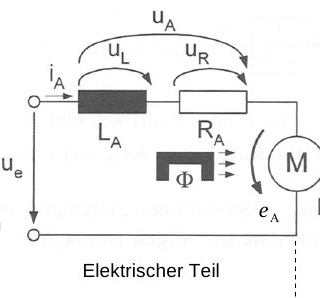
\includegraphics[width=0.6\textwidth]{ElektrischerTeil.jpg}
	\caption{Elektrischer Teil des Motors}
	\label{fig:elekeinzelteil}
\end{figure}
Es l�sst sich folgende Spannungsmasche aufstellen:
\begin{center}
\begin{equation}
\label{equ:motorspannung}
U_e = u_L + u_R - e_A
\end{equation}
\end{center}
Die Spannung $e_A$ wirkt der Eingangsspannung entgegen und hat ein negatives Vorzeichen.
Die Teilspannungen $u_L$ und $u_R$ lassen sich folgenderma�en umschreiben:
\begin{center}
\begin{equation}
\label{equ:motorersatzspannung}
u_L = L_A * si_A \\
u_R = R_A * i_A
s = \frac{d}{dt}
\end{equation}
\end{center}
Dieses l�sst sich in einer Formel ausdr�cken:
\begin{center}
\begin{equation}
\label{equ:motorspannungausfuehrlich}
U_e = L_A * si_A + R_A * i_A - e_A
\end{equation}
\end{center}
F�r die sp�tere Integration in Simulink wird die Gleichung \ref{equ:motorspannungausfuehrlich} umgeschrieben:
\begin{center}
\begin{equation}
\label{equ:motorspannungsimulink}
si_A = \frac{1}{L_A} (e_A - R_Ai_A + u_e)
\end{equation}
\end{center}
Wobei
\begin{center}
\begin{equation}
\label{equ:motorspannungsimulinkkonst}
e_a = K_M * \Phi \omega
\end{equation}
\end{center}
$K_M$ und $\Phi$ Motorkonstanten sind.

\subsection{Der mechanische Teil}
\label{chap:mechteil}
Der mechanische Teil eines Gleichstrommotors besteht aus dem gesamten Drehmoment $M_B$, dem Motormoment $M_M$, dem Lastmoment $M_L$ des Spiegels und der 
Moment-Winkel-Beziehung (Reibung) $M_R = r*\omega$, wobei $\omega = \.\phi$ ist, siehe Abb. \ref{mecheinzelteil}.
\begin{figure}[!h]
	\centering
	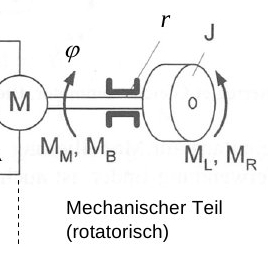
\includegraphics[width=0.6\textwidth]{MechanischerTeil.jpg}
	\caption{Mechanischer Teil des Motors}
	\label{fig:mecheinzelteil}
\end{figure}
Es l�sst sich folgende Moment-Bilanzgleichung aufstellen:
\begin{center}
\begin{equation}
\label{equ:motormomentebilanz}
M_B = M_M - M_R - M_L = \\
J * s\omega = M_M - r * \omega - M_L\\
s = \frac{d}{dt}
\end{equation}
\end{center}
F�r die sp�tere Integration in Simulink wird die Gleichung \ref{equ:motormomentebilanz} umgeschrieben:
\begin{center}
\begin{equation}
\label{equ:motormomentsimulink}
s\omega = \frac{1}{J} (M_M - r * \omega - M_L)
\end{equation}
\end{center}
Wobei
\begin{center}
\begin{equation}
\label{equ:motormomentsimulinkkonst}
M_M = K_M * \Phi *i_A
\end{equation}
\end{center}
$K_M$ und $\Phi$ Motorkonstanten sind.

\subsection{Der ganze Motor}
Werden die beiden Einzelaspekte des Motors gleichzeitig betrachtet, so ergbit sich folgender Zusammenhang wie er in Abb. \ref{fig:motoraufbau} dargestellt ist.
\begin{figure}[!h]
	\centering
	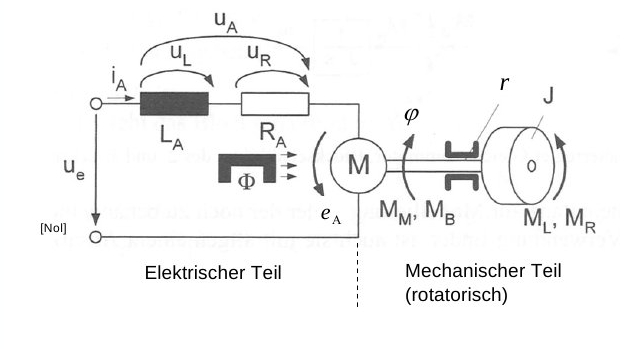
\includegraphics[width=0.6\textwidth]{Motoraufbau.jpg}
	\caption{Aufbau des Motors}
	\label{fig:motoraufbau}
\end{figure}

\section{Der Sensor}
\label{chap:sensor}
Im Folgenden werden der Aufbau, das physikalische Modell, sowie verschiedene mathematische Modelle des Sensors vorgestellt und erl�utert.

\subsection{Das physikalische Modell des Sensors}
\label{chap:physik_modell_sensor}
Der in Abb. \ref{fig:aufbau_system} dargestellte Sensor, gliedert sich nach folgender Darstellung in Abb. \ref{fig:aufbau_sensor} auf in:
\begin{itemize}
	\item{Einer Lichtquelle: LED mit einer Strahlungsleistung $\phi_e(\theta)$}
	\item{Einer Blende mit einer Transmissionsfunktion $T(\varphi)$}
	\item{Einer Anordnung aus Photodioden, welche die transmittierte Lichtleistung als Spannungssignal $U_{ph} (\phi)$ bzw. $U_{ph} (\varphi)$ darstellt}
\end{itemize}

\begin{figure}[ht]
	\centering
	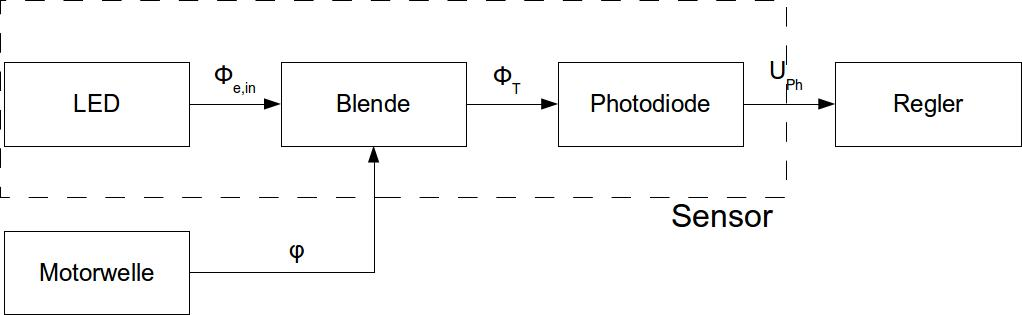
\includegraphics[width=0.8\textwidth]{Sensor_Aufbau.jpg}
	\caption{Allgemeiner Aufbau des Sensors}
	\label{fig:aufbau_sensor}
\end{figure}

\textbf{Die LED}\\
Die LED wird im folgenden als ein punktf�rmiger, lambert'scher Strahler betrachtet.
Die gesamte Strahlungsleistung $\phi_e$ wird in den Halbraum $\omega = 2\pi$ abgestrahlt. 
Das Spektrum der LED wird in dieser Simulationsstudie nicht ber�cksichtigt.\\
\textbf{Die Blende}\\
Die Blende wir im folgenden als masselos und v�llig lichtundurchl�ssig angenommen.

\begin{figure}[ht]
\centering
\subfigure[a]{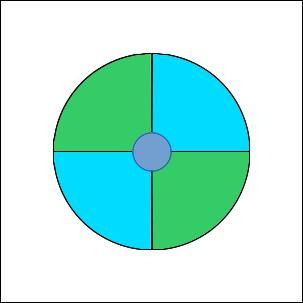
\includegraphics[height=45mm]{Sensor_DIODEN.jpg}}
\subfigure[b]{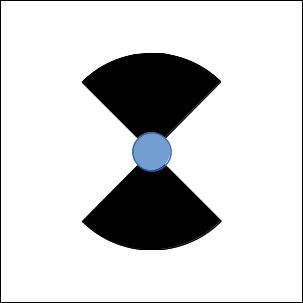
\includegraphics[height=45mm]{Sensor_BLENDE.jpg}}\vfill
\subfigure[c]{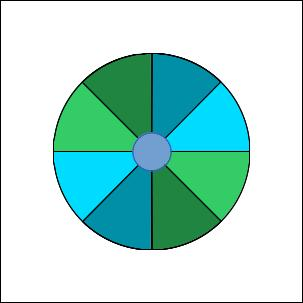
\includegraphics[height=45mm]{Sensor_Abdunklung_0.jpg}}
\subfigure[d]{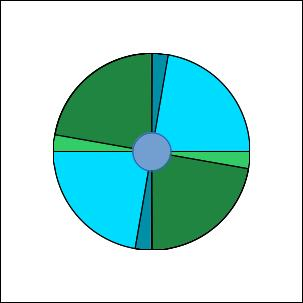
\includegraphics[height=45mm]{Sensor_Abdunklung_40.jpg}}
\caption{Sensor Funktions}
\label{abb:sensor_funktion}
\end{figure}




\subsection{Das lineare Sensormodell}
\label{chap:linear_sensor}


\subsection{Das nicht lineare Sensormodell}
\label{chap:nonlinear_sensor}